
\section{Introduction}
\label{sec:intro}

Internet privacy is a subset of data privacy and a fundamental human right as defined by the United Nations \cite{un2018}. In order to retain and exercise this right to privacy, each internet user must have full control of the transmission, storage, use, and disclosure of their personally identifiable information. However, the infrastructure and economics of our increasingly technologically driven world put great pressure on privacy, due to the various advantages (economic and otherwise) which knowledge of users' private information provides.

To combat this trend, multiple solutions are being developed to restore internet users' control of their private information. These solutions generally centre on providing truly anonymous communication, such that neither the content of the communication nor information about the communicators can be discovered by anyone, including the communicating parties.

HOPR is a decentralized incentivized mixnet \cite{mixnets} that employs privacy-by-design protocols. HOPR aims to protect users' transport-level metadata privacy, giving them the freedom to use online services safely and privately. HOPR leverages existing mechanisms such as the Sphinx packet format \cite{sphinxpaper} and packet mixing to achieve its privacy goals, but adds an innovative incentive framework to promote network growth and reliability. HOPR uses the Ethereum blockchain \cite{ethereum} to facilitate this incentive framework, specifically to perform probabilistic payments via payment channels.

\subsection{HOPR Design Ethos}
\label{sec:intro:vision}

HOPR is built with the following principles in mind: that privacy must be an integral part of the design process (privacy by design); that privacy cannot be reliably achieved in centralized systems; and that decentralized systems must be properly incentivized to provide privacy at a sufficient scale and level of reliability. The following section explains these three principles in more detail, as well as how HOPR meets them.

\subsubsection{Privacy by design}
Privacy by design is an approach to systems engineering which considers privacy throughout the entire engineering process, not merely as an afterthought. The internet is a public good – a digital commons that should be safe and secure to use for all users. However, it is impossible to provide such privacy using current internet infrastructure, which attaches little or no importance to metadata privacy, and indeed in many cases relies on copious amounts of metadata to be made public in order to function. Therefore, new infrastructure with a focus on privacy must be created on top of the existing internet. HOPR provides an essential part of that infrastructure, and has been built with privacy as its foremost goal.

\subsubsection{Decentralization}
The internet is not private by design, although it is decentralized by design. In the early days of the internet, this decentralization provided a certain measure of privacy, by placing control in the hands of individual users. However, internet users must increasingly interact with services provided by central authorities. These central authorities control the privacy of individual users, often without their full informed consent.

In particular, interactions with third-party service providers regularly entail a loss of transport-layer privacy. Links can often be drawn between the user and the service provider, either by the service provider themselves, or by a third party who can observe public metadata revealed during the interaction or pressure the service provider to divulge stored data. With a sufficient number of such links, a profile can be constructed of a user's online activity.

This runs contrary to the requirements of privacy as a fundamental human right, since often the only truly private option is to abstain from using such services entirely. To provide privacy as a fundamental feature on top of the internet, a decentralized infrastructure is required.

The HOPR protocol runs on nodes within a decentralized network, therefore ensuring that the network is independent. No single entity can influence its development or manipulate its performance to their advantage. It also makes the network resilient, able to keep running even if a majority of nodes are damaged or compromised and very difficult, if not impossible, to shut down.

\subsubsection{Incentivization}
Although users are incentivized to use privacy technologies by the privacy they provide, most privacy technologies have no baked-in incentive framework for infrastructure providers: rewards either flow to a centralized service provider (and thus the service is not truly private, since the service provider will gather transport-level information on user activity) or the providers in a decentralized network receive no direct rewards. This constrains the growth of the network and limits its scope. In systems which leverage privacy through obscurity, this reduced scale compromises the privacy of the entire network, since fewer users means less data to confound observers. Although blockchains provide a way, for the first time, to incentivize a decentralized network without introducing a centralized entity responsible for payment provision, it is challenging to leverage blockchain technology without compromising either the privacy of network members or the reliability of the network. In brief, if node runners can rely on the anonymity of the technology they are providing, they can potentially use it to claim rewards without properly fulfilling their duties as a node runner. On the other hand, if node runners are required to interact with a blockchain to prove their service provision and claim their reward, the resultant on-chain data is liable to provide a permanent and growing source of metadata which can be used to erode the users' privacy.

HOPR's proof-of-relay mechanism threads this needle, and is the major innovation of the HOPR protocol. Every HOPR node can receive payment for each packet they process and forward, but only once their data payload arrives at the next node. Payments are probabilistic and cheat-proof, which ensures nodes do not (de-)prioritize other nodes and/or packets. To maximize received incentives, node operators must ensure good network connectivity, node availability, computational capacity, and committed funds (to reward other nodes). These combined incentives promote a broad, robust, and reliable network. At the same time, the probabilistic nature of payments obscures links between on-chain data and node runners.


\subsection{Security Goals}
\label{sec:intro:securitygoals}

Generally, the HOPR protocol aims to hide the fact that two parties are communicating with each other, as well as the contents of the communication. This information should be hidden from any party external to the network, all intermediaries involved in transferring the data between the communicating parties, and even the communicating parties themselves, if one or both of them desires it.

Specifically, the HOPR protocol aims to build a network with the following features (definitions based on \cite{AnoA}, \cite{loopix} and \cite{sphinxpaper}) for senders, indicated by $A_n$ and recipients, indicated by $Z_n$.

\subsubsection{Sender anonymity}
In a network with sender anonymity, an observer is not able to tell if a particular packet was sent by any adversary-selected honest senders $A_1$ or $A_2$ to the honest recipient $Z$. Formally this is denoted as $\{A_1 \rightarrow Z, A_2 \not\rightarrow \}$ or $\{A_1 \not\rightarrow, A_2 \rightarrow Z \}$.

\subsubsection{Recipient anonymity}
In analogy to sender anonymity, here an observer is not able to tell if a particular packet was received by any adversary-selected honest recipients $Z_1$ or $Z_2$ from the honest sender $A$. Formally this is denoted as $\{A \rightarrow Z_1, \not\rightarrow Z_2 \}$ or $\{\not\rightarrow Z_1, A \rightarrow Z_2 \}$.

\subsubsection{Sender-recipient unlinkability}
For any pair of senders, $A_1$ and $A_2$, communicating with any pair of recipients, $Z_1$ and $Z_2$, an adversary must be unable to determine whether two packets travelled from $\{A_1 \rightarrow Z_1, A_2 \rightarrow Z_2 \}$ or $\{A_1 \rightarrow Z_2, A_2 \rightarrow Z_1 \}$.


These properties assume senders and recipients are honest, but they should hold for any honest senders and recipients of the adversary's choice.

To provide these features, the HOPR protocol builds on top of the Sphinx packet format \cite{sphinxpaper}, the specifics of which are explained in Section \ref{sec:sphinx}. HOPR also employs cover traffic, explained in Section \ref{sec:CT}. The additional parameters required for HOPR's incentive scheme are encapsulated in the Sphinx header as described in section \ref{sec:incentives:proofofrelay:challenge} as additional routing parameters and as such do not change the privacy guarantees of Sphinx.


\subsection{Threat Model}
\label{sec:intro:threatmodel}

Although we assume that nodes in the HOPR network can communicate reliably, the network must still be protected from malicious actors and node failures. We assume a threat model with Byzantine nodes with the ability to either observe all network traffic and launch network attacks or to inject, drop, or delay packets as follows:

\subsubsection{Global passive adversaries (GPAs)} A global passive adversary (GPA) is an attacker who can observe the entirety of network traffic passing between users. A GPA is considered passive because their attacks are based on observation alone. A theoretical GPA is arbitrarily powerful, and their full abilities are unlikely to be manifest in any real-world attacker. Nonetheless, building a network which is GPA-resistant introduces extra security through redundancy and future-proofing.

Thanks to the properties of Sphinx (see Section \ref{sec:sphinx}) and proof of relay (see Section \ref{sec:incentives:proofofrelay}), HOPR is able to defend against GPAs. Nonetheless, it is worth mentioning some additional attacks that a decentralized mixnet like HOPR is particularly vulnerable to by virtue of its decentralized and anonymous nature.

\subsubsection{Sybil attacks}
In a Sybil attack, an attacker forges multiple identities in the network, thereby introducing network redundancy and reducing system security. The attacker can potentially de-anonymize packet traffic and thus link the sender and recipient's identities. HOPR mitigates Sybil attacks via the trust assumption of the Sphinx packet format: only a single honest relayer is needed to ensure integrity of the entire transmission chain, and since the traffic is source routed, users can choose routes themselves to ensure this minimal requirement of one honest relayer is met. Since path selection is dependant on a financial stake, launching a Sybil attack would be prohibitively expensive.

\subsubsection{Eclipse attacks}
Many decentralized networks suffer from a general unavailability of a general understanding of their topology, hence nodes cannot determine whether their respective local views are complete or accurate. As an attacker, it might be attractive to flood a victim with inaccurate information about collaborating nodes while withholding information about honest nodes.

HOPR mitigates this issue by using a different medium to announce entry nodes to the network. This is done using a smart contract on a blockchain and known within HOPR as DEADR (Decentralized Entry Advertisement and Distributed Relaying). DEADR nodes serve two functions: (1) providing access to the distributed hash table (DHT) that is used within the libp2p environment that HOPR leverages and (2) facilitating network address translation (NAT) or relaying traffic that cannot be sent directly between adjacent nodes who reside in separate internet sub-networks (e.g., computers without a public internet-facing internet protocol (IP) address behind typical home routers). A HOPR node only requires access to one honest DEADR node and it is significantly cheaper in computational terms to check whether a DEADR node is honest than to conduct an eclipse attack, which requires on-chain transactions. A successful eclipse attack therefore requires controlling all announced DEADR nodes or forging a public blockchain, both of which we assume are impossible and beyond the scope of this work.

Thus we are satisfied that HOPR more than adequately protects users against attack. However, security cannot come at the expense of usability. To be appealing to users and node runners alike, it is important for HOPR to find a satisfactory compromise to what is known as the ``anonymity trilemma" \cite{AnonymityTrilemma}, which states that a privacy network can provide at most two of the following properties: low latency communication, low bandwidth overhead, and strong anonymity.

The rest of this paper will outline the current state of the art among anonymous communication protocols and layer-2 scalability protocols, describe how the HOPR network is built, and explain how HOPR provides a satisfactory resolution to the anonymity trilemma.

\subsection{State of the Art}
\label{sec:intro:stateoftheart}

HOPR has been built on top of, or as a reaction to, various technologies and research projects which try to meet some or all of the design ethos and security goals outlined above. These technologies and research projects can be broadly divided into three groups: (1) \lcnameref{sec:intro:stateoftheart:privacyprotocols} which attempt to hide user information; (2) \lcnameref{sec:intro:stateoftheart:l2protocols} which allow systems to perform micro-payments via the Ethereum blockchain, as well as (3) \lcnameref{sec:intro:stateoftheart:p2pnetworks} which allow nodes to interact with each other directly without requiring a central coordinator. The following sections present the state of the art for each of these groups.

\subsubsection{Anonymous Communication Protocols}
\label{sec:intro:stateoftheart:privacyprotocols}

\paragraph{Virtual Private Networks}(\textit{VPNs}) are point-to-point overlay networks used to create secure connections over an otherwise untrusted network, such as the internet \cite{venkateswaran_2001}. Clients receive a public IP address from the VPN endpoint, which is then used for all outgoing communication. Since this public IP address can be almost anywhere in the world, VPNs are often used to bypass censorship \cite{hobbs_roberts_2018} and geolocalization blocks. However, VPNs provide dubious privacy, since clients must trust the VPN endpoint. The endpoint provider has full access to users' connection and communication metadata, since they control all communication going through it. In addition, VPN endpoints are often a single point of failure, since they are provided as centralized services. Both factors are major weaknesses when considering VPNs for privacy-preserving communication.

These privacy concerns have motivated the creation of a new model for VPNs, \textbf{Decentralized Virtual Private Networks} (\textit{dVPN}s). dVPNs leverage blockchain technology to remove reliance on a central authority. Users act as bandwidth providers, allowing other users to access internet services via their node, in exchange for rewards.

Examples of dVPN projects include Orchid \cite{orchid}, Sentinel \cite{sentinel}, and Mysterium \cite{mysterium}. However, these projects still lack privacy, performance, and reliability guarantees, since bandwidth providers can potentially inspect, log, and share any of their traffic. This harms honest bandwidth providers as well as users: since bandwidth providers can theoretically monitor traffic, nodes whose bandwidth are used to enable illicit activity can potentially be held liable for those activities by government authorities. Indeed, there have been incidents where unaware dVPN users have been (ab)used as exit nodes through which DDoS attacks
were performed.

A research project called VPN$^0$ \cite{vpn0} aims to provide better privacy guarantees. VPN$^0$ leverages zero-knowledge proofs to hide traffic content to relay nodes with traffic accounting and traffic blaming capabilities as a way to combat the weaknesses of other dVPN solutions.

\paragraph{Onion Routing} is another approach to network privacy, implemented by projects such as Tor \cite{tor}. Tor encapsulates messages in layers of encryption and transmits them through a series of network nodes called \textit{onion routers}. However, Tor is susceptible to end-to-end correlation attacks from adversaries who can eavesdrop on the communication channels. These attacks reveal a wide range of information, including the identity of the communicating peers.

The Invisible Internet Project (\textit{I2P}) is an implementation of onion routing with notably different characteristics than Tor \cite{i2p}:

\begin{itemize}

      \item \textbf{Packet switched instead of circuit switched}
            Tor allocates connection to long-lived circuits; this allocation does not change until either the connection or the circuit closes. In contrast, routers in I2P maintain multiple tunnels per destination. This significantly increases scalability and failure resistance since packets are used in parallel.

      \item \textbf{Unidirectional tunnels}
            Employing unidirectional rather than bidirectional tunnels makes deanonymization harder, because tunnel participants see half as much data and need two sets of peers to be profiled.

      \item \textbf{Peer profiles instead of directory authorities}
            I2P’s network information is stored in a DHT (information in the DHT is inherently untrusted) while Tor’s relay network is managed by a set of nine Directory Authorities.
\end{itemize}

Despite these improvements, I2P is vulnerable to eclipse attacks since no I2P router has a full view of the global network (similar to other peer-to-peer networks). Like Tor, I2P only provides protection against local adversaries, making it vulnerable to timing, intersection, and traffic analysis attacks. I2P has also been shown to be vulnerable to Sybil and predecessor attacks, in spite of various countermeasures implemented to thwart these.

\paragraph{Mixnets} are overlay networks of so-called \textit{mix nodes} which route packets anonymously, similarly to Tor \cite{mixnets}. Mixnets originally used a cascade topology where each node would receive a batch of encrypted messages, decrypt them, randomly permute packets, and transfer them in parallel. Cascade topology makes it easy to prove the anonymity properties of a given mixnet design for a particular mix. However, it does not scale well with respect to increasing mixnet traffic and is susceptible to traffic attacks. Since then, research has evolved to provide solutions with low latency while still providing high anonymity by using a method called \textit{cover traffic}. Cover traffic is designed to hide communication packets among random noise. An external adversary able to observe the packet flow should not be able to distinguish communication packets from these cover traffic packets, increasing privacy.

The application of cover traffic provides metadata protection from global network adversaries, a considerable improvement on projects such as Tor and I2P. However, because mixnets add extra latency to network traffic, they are better suited to applications that are not as sensitive to increased latency, such as messaging or email applications. For applications such as real-time video streaming, Tor may be more suitable, provided the user feels the latency improvements outweigh the increased privacy risks.

Loopix \cite{loopix} is another research project which uses cover traffic to resist traffic analysis while still achieving low latency. To achieve this, Loopix employs a mixing strategy called \textit{Poisson mix}. Poisson mix nodes independently delay packets, making packets unlinkable via timing analysis.

\subsubsection{Layer-2 Scalability Protocols}
\label{sec:intro:stateoftheart:l2protocols}

Blockchain technology (mostly public blockchains like Bitcoin and Ethereum) suffers from a major scalability issue: every node in the network needs to process every transaction, validate them, and store a copy of the entire chain state. Thus the number of transactions cannot exceed that of a single node. For Ethereum, this is currently around 30 transactions per second.

Multiple solutions have been proposed to resolve the scalability issue, including sharding and off-chain computation. Both approaches intend to create a second layer of computation to reduce the load on the blockchain mainnet.

Off-chain solutions such as Plasma \cite{plasma}, Truebit \cite{truebit}, and state channels process transactions outside the blockchain while still guaranteeing a sufficient level of security and finality. State channels are better known as ``payment channels". In models like the Lightning Network \cite{lightningnetwork}, a payment channel is opened between two parties by committing a funding transaction. Those parties may then make any number of signed transactions that update the channel's funds without broadcasting those to the blockchain. The channel is eventually closed by broadcasting the final version of the settlement transaction. The channel balance is updated by creating a new set of commitment transactions, followed by trade revocation keys which render the previous set of commitment transactions unusable. Both parties always have the option to ``cash out" by submitting the latest commitment transaction to the blockchain. If one party tries to cheat by submitting an outdated commitment transaction, the other party can use the corresponding revocation key to take all the funds in the channel.

As soon as closure is initiated, the channel can no longer be used to route payments. There are different channel closure transactions depending on whether both parties agree on closing the channel. If both agree, they provide a digital signature that authorizes this cooperative settlement transaction. In the case where they disagree or only one party is online, a unilateral closure is initiated without the cooperation of the other party. This is done by broadcasting a ``commitment transaction". Both parties will receive their portion of the money in the channel, but the party that initiates the closure must wait for a certain delay to receive their money. This delay time is negotiated by the nodes before the channel is opened, for the protection of both parties.

The Raiden network \cite{raiden} is a layer-2 payment solution for the Ethereum blockchain. The project employs the same technological innovations pioneered by the Bitcoin Lightning Network by facilitating transactions off-chain, but provides support for all ERC-20 compliant tokens. Raiden differs in operation from its main chain because it does not require global consensus. However, to preserve the integrity of transactions, Raiden powers token transfers using digital signatures and hash-locks. Known as \textbf{balance proofs}, this type of token exchange uses payment channels. Raiden also introduces ``mediated transfers", which allow nodes to send payments to another node without opening a direct channel to it. These payment channels are updated with absolute amounts, whereas HOPR employs relative amounts (more details in Section \ref{sec:tickets}).

\begin{comment}
We present in the following a comparison table (from the Loopix paper) between different anonymous communication systems.

\begin{figure}[H]
      \centering
      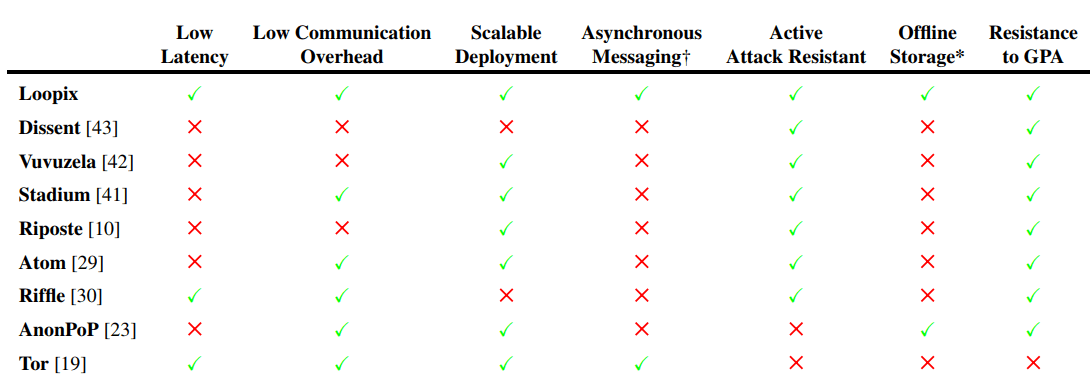
\includegraphics[width=11cm,height=11cm,keepaspectratio]{../yellowpaper/images/state-of-the-art.png}
      \caption{Comparison between anonymous communication systems}
      \label{fig:Comparison between anonymous communication systems}
\end{figure}
\end{comment}

\subsubsection{Decentralized Networks}
\label{sec:intro:stateoftheart:p2pnetworks}

Many, if not most, services in the internet implement the client-server principle in which the client requests resources from the server which acts as a single source of truth. This principle does not only establish a clear hierarchy between both parties, allowing the server to fully control the state that is observable by the client, but also introduces single points of failure in the network [add Facebook outage].

TODO: add decentralization picture

\paragraph{P2P Networking}

When applying the client-server principle, clients usually do not connect directly. Instead, they establish a direct connection to the server and the server forwards the data to other clients. In this setting, it is the responsability of the server to reachable for the client and the responsibility of the client to find a way to connect to the server.

As Peer-to-Peer (P2P) networks aim to forego the usage of a central server, each node needs to fulfill both roles and thus needs to remain reachable by other nodes and determine a means of communication to other nodes. As of now, this is usually done using version four of the Internet Protocol (IPv4). It is expected to switch to version six of the Internet Protocol (IPv6) due the scarcity of IPv4 addresses but the transformation process has not yet reached a point where the majority of nodes can connect to each other using IPv6.

Due to the aforementioned scarcity of IPv4 addresses, it is a common principle to led many machines share the same IPv4 address by using a Network Address Translation (NAT) mechanism that maps local addresses to one or more public IP addresses by rewriting the source port of outgoing packets and the destination port of incoming packets. In general, this mapping is not static. Thus, nodes need add to add on demand an entry to the address mapping in order to receive messages from outside their local network. This makes it complicated for nodes in a local network to be reachable by other nodes.

Figure \ref{fig:successful-nat-traversal} shows two nodes, \textit{A} and \textit{B} that are connected to the internet through a router that applies a NAT mechanism. As both routers transparently rewrite the source port, node \textit{A} needs to know to which external port node \textit{B} is mapped by their router in order to deliver data. To establish a duplex connection, node \textit{B} needs to know \textit{A}'s external port.

\begin{figure}[H]
      \centering
      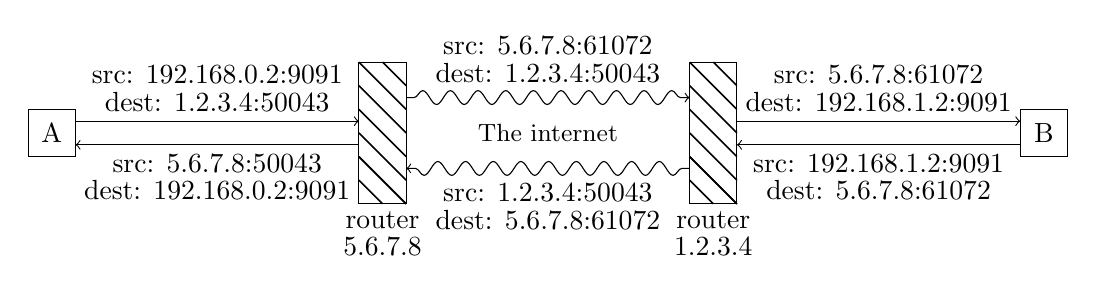
\begin{tikzpicture}
            \def\nodeWidth{0.6}
            \def\nodeHeight{0.6}
            \def\routerWidth{0.6}
            \def\routerHeight{1.8}
            \def\routerOffset{4.2}

            % Subnet A
            \draw (0,0) rectangle (\nodeWidth,\nodeHeight) node[midway] {A};

            % Interaction with router A
            \draw[->] (\nodeWidth,0.75*\nodeHeight) -- (\routerOffset,0.75*\nodeHeight) node[midway,above] {\smaller{\shortstack{src: 192.168.0.2:9091\\dest: 1.2.3.4:50043}}};

            \draw[->] (\routerOffset,0.25*\nodeHeight) -- (\nodeWidth,0.25*\nodeHeight) node[midway,below] {\smaller{\shortstack{src: 5.6.7.8:50043\\dest: 192.168.0.2:9091}}};

            % Router to router interaction
            \begin{scope}[shift={(0,-0.6)}]
                  \draw[->,decorate,decoration={snake,pre length=1mm,post length=1mm}] (\routerOffset+\routerWidth,0.75*\routerHeight) -- (2*\routerOffset,0.75*\routerHeight) node[midway,above=2pt] {\smaller{\shortstack{src: 5.6.7.8:61072\\dest: 1.2.3.4:50043}}};
                  \draw[->,decorate,decoration={snake,pre length=1mm,post length=1mm}] (2*\routerOffset,0.25*\routerHeight) -- (\routerOffset+\routerWidth,0.25*\routerHeight) node[midway,below=2pt] {\smaller{\shortstack{src: 1.2.3.4:50043\\dest: 5.6.7.8:61072}}};

                  \path (\routerOffset+\routerWidth,0.5*\routerHeight) -- (2*\routerOffset,0.5*\routerHeight) node[midway] {\small{The internet}};
            \end{scope}

            % Subnet B
            \begin{scope}[shift={(3*\routerOffset,0)}]
                  \draw (0,0) rectangle (\nodeWidth,\nodeHeight) node[midway] {B};
                  % Interaction with router B
                  \draw[->] (-\routerOffset+\routerWidth,0.75*\nodeHeight) -- (0,0.75*\nodeHeight) node[midway,above] {\smaller{\shortstack{src: 5.6.7.8:61072\\dest: 192.168.1.2:9091}}};

                  \draw[->] (0,0.25*\nodeHeight) -- (-\routerOffset+\routerWidth,0.25*\nodeHeight) node[midway,below] {\smaller{\shortstack{src: 192.168.1.2:9091\\dest: 5.6.7.8:61072}}};
            \end{scope}

            \foreach \offset\name\address in{1/A/5.6.7.8,2/B/1.2.3.4} {
                        \begin{scope}[shift={(\offset*\routerOffset,-0.6)}]
                              \def\a{0.6}
                              \def\b{1.8}
                              \def\diff{1.2}

                              \def\lw{0.2}

                              \foreach \x [count=\i] in{0,0.3,0.6,...,\a}{
                                          \draw [line width=\lw mm](\x,0)--(0,\x) (\x,\b)--(\a,\b-\a+\x);
                                    }
                              \foreach \x [count=\i] in{0,0.3,0.6,...,\diff}{
                                          \draw [line width=\lw mm](0,\a+\x)--(\a,\x);
                                    }
                              \draw (0,0) rectangle  node[below=25pt] {\smaller{\shortstack{router\\\address}}} (\routerWidth,\routerHeight);
                        \end{scope}

                  }
      \end{tikzpicture}
      \label{fig:successful-nat-traversal}
      \caption{Network address translation done by most routers.}
\end{figure}

As of this, it is key for traversing NATs to find out (1) if and if yes, (2) to which external port their connection is mapped and (3) if the mapping is done individually for each destination address and if in this case, (4) the NAT follows any observable pattern. Depending on which NAT mechanism the router implements, nodes can either establish a direct connection or fallback to a relayed connection using the TURN protocol.

If possible, establishing a direct connection is done in general using ICE protocol together with one or more STUN servers and a signalling server that acts as a rendezvous point and allows nodes to exchange connection information.

\paragraph{Distributed Hash Tables}

% DHT 

% NAT Traversal
\subsection{Assessment}
\label{sec:intro:assessment}

Although there are numerous projects attempting to solve the problem of online privacy, most fail to satisfy the design principles and security goals outlined in Section \ref{sec:intro:securitygoals}.

\paragraph{Privacy} The metadata privacy properties that a mixnet like HOPR provides are significantly beyond what VPNs, dVPNs, or even Tor can deliver. VPNs and dVPNs have single points of trust and failure. Tor and I2P have been shown to be subject to a large variety of de-anonymizing attacks, which a mixnet like HOPR is resilient against. The HOPR mixnet unlinks sender and recipient even when faced by powerful global passive adversaries (GPAs) which can monitor every packet in the network. This is achieved by packet transformation, mixing, and introducing delays before forwarding a packet, as well as bandwidth overhead in form of cover traffic and packet padding.

\paragraph{Decentralization} Most projects presented above have decentralization as a core goal (with the exception of VPNs, where the service is provided by a centralized entity, at the expense of user privacy). However, many projects lack the impetus to scale, which prevents them from leveraging many of the advantages which come with a decentralized network, such as privacy through obscurity, while retaining all of the challenges, such as coordination and consensus issues. It is our opinion that the only way to solve the scalability problem is with the introduction of a robust incentivization scheme for node runners.

\paragraph{Incentivization} Many projects referenced in this section lack incentivization of any kind. VPNs incentivize the service provider, but since this is a centralized entity this fails the privacy condition.

Bandwidth providers in dVPNs share their resources and are granted tokens accordingly as payment for their services. For example, Mysterium \cite{mysterium}, an open-source dVPN built on top of a P2P architecture, uses a smart contract on top of Ethereum to ensure that the VPN service is adequately funded. However, the resultant liability risk for dVPNs means these incentives are likely to be insufficient.

Tor and I2P rely on donations and government funding, which only covers the cost of running a node, not any additional reward. This has discouraged volunteers from joining these networks and the number of relayers in both networks has stayed mostly static in recent years, even as usage and the demand for privacy has risen sharply.

Mixnet designs are generally unconcerned with the problem of incentivization, and most existing implementations rely on a group of volunteer agents who lack incentives to participate. However, it is possible to add incentivization on top of a mixnet design, which is what HOPR does. Some authors have proposed adding digital coins to packet delivery in mixnets \cite{MixnetCoins}. However, here the anonymity provided by the mixnet acts as a double-edged sword: since there is no verification for whether a packet arrives at its final destination, and node identities are kept secret by the mixnet, selfish nodes can extract payment without performing their relaying task or without passing on acknoledgements to the next node. Thus a naive implementation of this approach does not actually provide an incentive at all.

It is in this last area that HOPR provides its main innovation: HOPR's proof-of-relay mechanism ensures that node runners are only paid if they complete their relaying duties. The challenge is to enforce this without publicizing data which would allow an adversary to break the anonymity of the network, and to provide both incentivization and anonymity without introducing unacceptable latency and bandwidth costs. The remainder of this paper will explain how this is achieved.
